\documentclass[a4paper,12pt]{article}
\usepackage[french]{babel} 
\usepackage[T1]{fontenc}
%\usepackage[ansinew]{inputenc}
\usepackage[utf8]{inputenc}
\usepackage[top=3cm, bottom=3cm, left=2.3cm,right=2cm]{geometry}
\usepackage{graphicx}
\usepackage{color}
\usepackage{listings}
%\usepackage{marvosym}
%\usepackage{yfonts}
\usepackage[normalem]{ulem}
\usepackage{verbatim}
\usepackage{listings}
\usepackage{float}
%\renewcommand{\thesection}{\arabic{section}}
\usepackage{array} % pour les tableaux
\usepackage{amsmath} % pour les équations
\usepackage{float}
\usepackage{hyperref}	% crée des liens dans le pdf
\hypersetup{					% colorise les liens du pdf
  colorlinks=true,
  urlcolor=black
	citecolor=black,
  linkcolor=black,
  urlcolor=blue
}
\usepackage{url}			% change la police des url (utilisation : \url{http://asdf.ch})
\definecolor{dkgreen}{rgb}{0,0.6,0}
\definecolor{gray}{rgb}{0.5,0.5,0.5}
\definecolor{mauve}{rgb}{0.58,0.01,0.82}
%[babel=true]
\usepackage{csquotes}
\lstset{ %
  language=C,                % the language of the code
  basicstyle=\footnotesize,           % the size of the fonts that are used for the code
  numbers=left,                   % where to put the line-numbers
  numberstyle=\tiny\color{gray},  % the style that is used for the line-numbers
  stepnumber=1,                   % the step between two line-numbers. If it's 1, each line 
                                  % will be numbered
  numbersep=5pt,                  % how far the line-numbers are from the code
  backgroundcolor=\color{white},      % choose the background color. You must add \usepackage{color}
  showspaces=false,               % show spaces adding particular underscores
  showstringspaces=false,         % underline spaces within strings
  showtabs=false,                 % show tabs within strings adding particular underscores
  frame=single,                   % adds a frame around the code
  rulecolor=\color{black},        % if not set, the frame-color may be changed on line-breaks within not-black text (e.g. commens (green here))
  tabsize=2,                      % sets default tabsize to 2 spaces
  captionpos=b,                   % sets the caption-position to bottom
  breaklines=true,                % sets automatic line breaking
  breakatwhitespace=false,        % sets if automatic breaks should only happen at whitespace
  title=\lstname,                   % show the filename of files included with \lstinputlisting;
                                  % also try caption instead of title
  keywordstyle=\color{blue},          % keyword style
  commentstyle=\color{dkgreen},       % comment style
  stringstyle=\color{mauve},         % string literal style
  escapeinside={\%*}{*)},            % if you want to add a comment within your code
  morekeywords={*,...}               % if you want to add more keywords to the set
}


%en-tête
\usepackage{fancyhdr}
\lhead{CSEL}
\chead{}
\rhead{\today}
\pagestyle{fancy}

% Title Page
\title{\Huge{\textsc{Systèmes d'exploitation mobiles et applications}} \\ 
\Huge{\textbf{TP01 - To Do List}} \\
\huge{Master HES-SO}}
\author{Émilie \textsc{Gsponer}, Grégory \textsc{Emery} }
\date{\today \\
version 1.0}

%-------------------------début du document-------------------------------------
\begin{document}

\maketitle % page de garde

\tableofcontents % table des matières
\setlength\parindent{0pt}
\newpage 
\section{Introduction}
\subsection{Cas pratique}
Dans ce travail pratique, nous devons créer une application permettant de gérer une To Do List. Deux vues seront créées. L'application pourra naviguer entre les deux.\\
Dans la première vue, on retrouve une représentation des tâches
existantes. Chaque entrée est constituée d’une image (« ! » ou vide ) ainsi que d’un descriptif de
la tâche.\\
L'autre vue permet l’ajout d’une nouvelle tâche dans la liste. Un bouton sert à indiquer si la tâche est urgente ou non, un champ de text permet de recevoir le nom de la tâche.\\
L'image ci-dessous présente la solution de design proposée par la donnée.
\begin{figure}[H]
	\begin{center}
		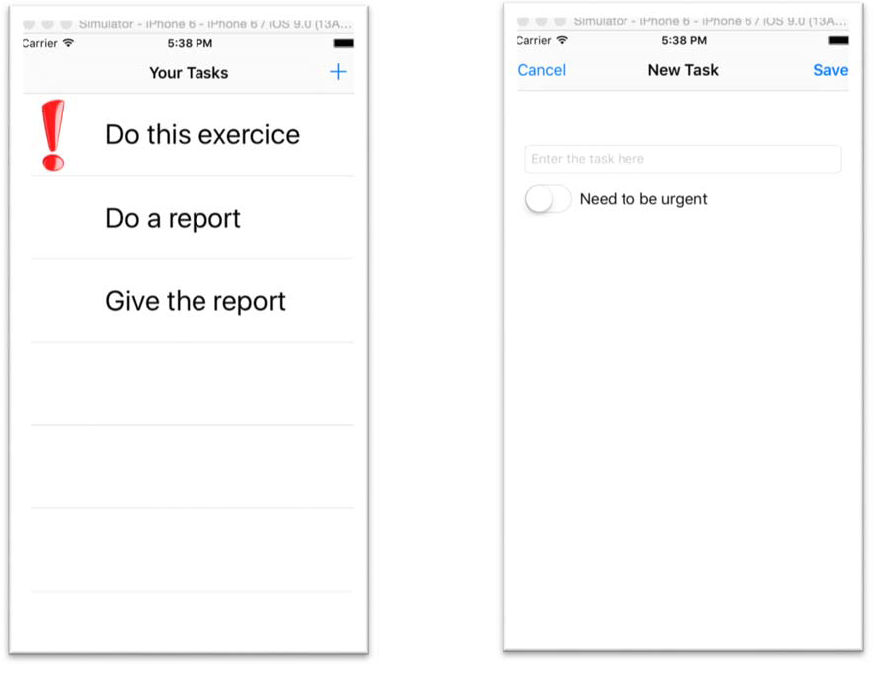
\includegraphics[width=10cm]{img/intro.png}
		\caption{Vues de l'application}
		\label{intro}
	\end{center}
\end{figure}

\subsection{Buts}
\begin{enumerate}
	\item Se familiariser avec le langage swift
	\item Utilisation de "Navigation Controller"
	\item Comprendre le développement et déploiement d'application iOS.
\end{enumerate}

\subsection{Objectifs}
\begin{enumerate}
	\item Création de la vue pour l’ajout d’une tâche
	\item Connecter la vue avec le "view controller" pour l’ajout et implémenter le contrôleur.
	\item Création du modèle qui représente une tâche
	\item Création de la vue pour lister les tâches
	\item Connecter la vue avec le "table view controller" pour la gestion de la table et implémenter le contrôleur
	\item  Mise en place de la navigation
\end{enumerate}
\section{Travail réalisé}
Tous les points exigés par la donnée ont été réalisés. Les éléments suivants ont fait l'objet d'une recherche approfondie et ont été utilisés dans le projet:
\begin{enumerate}
	\item Stackview : équivalent aux LinearLayout d'Android
	\item View controller : gère la navigation entre les vues
	\item Optional types : si une variable n'est pas initialisée, elle contient nil
	\item Table view : équivalent aux ListView d'Android
	\item Protocol UITextFieldDelegate : Interface proposant des méthodes gérant le champ de texte.
	\item unwind segue : permet de quitter une vue et de revenir à une autre en appelant une méthode spécifique de cette dernière.\\
\end{enumerate}
Cette image représente les deux vues de l'application développée.
\begin{figure}[H]
	\begin{center}
		\includegraphics[width=14cm]{img/simulator.png}
		\caption{Vues de l'application réalisée}
		\label{vues}
	\end{center}
\end{figure}
\textbf{Source de l'image !:\\}
\url{http://static.guim.co.uk/sys-images/Guardian/Pix/pictures/2009/4/29/1240996556472/exclamation-001.jpg}\\\\
\textbf{N.B :} A cause de l'implémentation du protocole UITextFieldDelegate, il est impératif d'appuyer sur la touche retour du clavier après avoir entrée le nom de la tâche. Sans cela, le bouton save ne devient pas actif.
\section{Problèmes rencontrés}
Un "bug" s'est produit avec XCode. Il y avait deux versions différentes du même fichier .swift dans le projet pour une raison inconnue. Le storyboard en affichait une et le projet en compilait une autre. Ce problème nous a fait perdre beaucoup de temps. Il a été découvert en introduisant une erreur dans le fichier et le projet compilait quand même. Le problème a été résolu en copiant le même code dans les deux versions.
\section{Réponse aux questions}
\subsection{Question 1}
\textbf{Donnée: }Expliquez avec vos mots, quelle est l’utilité d’identifier la segue.\\\\
Dans le projet, on a utilisé des segues "identifiées" dans les méthodes preparForSegue. Cela a permis en fonction de quelle segue a déclenché l'action de passer ou non des informations à la prochaine vue.

\subsection{Question 2}
\textbf{Donnée: }Expliquez l’utilité d’une « unwind segue ».\\\\
Elle permet de quitter une vue et de revenir simplement à une autre en appelant une méthode spécifique de cette dernière. L'avantage est que l'on sait exactement à quel endroit du code on revient dans l'autre vue, cela permet de faire une action spécifique comme par exemple mettre à jour le contenu d'une TableView.

\subsection{Question 3}
\textbf{Donnée: }Expliquez avec vos mots, qu’est-ce qu’une structure.\\\\
Une structure est semblable à une énumération. Ses propriétés sont semblables aux classes. Le différence est que la struct fonctionne par copie alors que les classes utilisent des références.

\subsection{Question 4}
\textbf{Donnée: }Expliquez le principe de « Convenience » avec vos propres mots.\\\\
Le mot clé convenience est utilisé pour les initialisations de classes. Cela permet d'offrir à l'utilisateur plusieurs manière d'initialiser la classes en passant un nombre de paramètres variables et définir des valeurs par défaut. Voici un exemple plus parlant:
\begin{lstlisting}
init(content: String, sender: String, recipient: String)
{
	self.content = content
	//Rule 1:  Calling designated Initializer from immediate superclass
	super.init(sender: sender, recipient: recipient)
}
convenience init()
{
	//Rule 2:  Calling another initializer in same class
	self.init(content: "")
}
convenience init(content: String)
{
	//Rule 2:  Calling another initializer in same class
	self.init(content: content, sender: "Myself")
}
convenience init(content: String, sender: String)
{
	//Rule 2 and 3:  Calling the Designated Initializer in same class
	self.init(content: content, sender: sender, recipient: sender)
}
\end{lstlisting}
\section{Conclusion}
Ce projet a permis de constaté que le support en ligne pour le développement sur iOS avec Swift est moins bien fournie qu'avec Android, il y a moins de tutoriels. Cela vient surement du fait que la programmation était auparavant en Objective C, la plupart des exemples trouvés sont dans ce langague et non en Swift.\\
Une autre observation est que l'implémentation du MediaPlayer est relativement simple et ne demande pas beaucoup de code. Les boutons play,stop... sont déjà implémentés.

\end{document}


